\documentclass{Configuration_Files/PoliMi3i_thesis}

%------------------------------------------------------------------------------
%	REQUIRED PACKAGES AND  CONFIGURATIONS
%------------------------------------------------------------------------------

% CONFIGURATIONS
\usepackage{parskip} % For paragraph layout
\usepackage{setspace} % For using single or double spacing
\usepackage{emptypage} % To insert empty pages
\usepackage{multicol} % To write in multiple columns (executive summary)
\usepackage{listings} % For code highlighting
\usepackage{xcolor}   % For syntax highlighting colors
\usepackage{geometry} % For custom margins
\usepackage{amsmath}
\geometry{margin=1in}
\setlength\columnsep{15pt} % Column separation in executive summary
\setlength\parindent{0pt} % Indentation
\raggedbottom  

% PACKAGES FOR TITLES
\usepackage{titlesec}
% \titlespacing{\section}{left spacing}{before spacing}{after spacing}
\titlespacing{\section}{0pt}{3.3ex}{2ex}
\titlespacing{\subsection}{0pt}{3.3ex}{1.65ex}
\titlespacing{\subsubsection}{0pt}{3.3ex}{1ex}
\usepackage{color}

% PACKAGES FOR LANGUAGE AND FONT
\usepackage[english]{babel} % The document is in English  
\usepackage[utf8]{inputenc} % UTF8 encoding
\usepackage[T1]{fontenc} % Font encoding
\usepackage[11pt]{moresize} % Big fonts

% PACKAGES FOR IMAGES
\usepackage{graphicx}
\usepackage{transparent} % Enables transparent images
\usepackage{eso-pic} % For the background picture on the title page
\usepackage{subfig} % Numbered and caption subfigures using \subfloat.
\usepackage{tikz} % A package for high-quality hand-made figures.
\usetikzlibrary{}
\graphicspath{{./Images/}} % Directory of the images
\usepackage{caption} % Coloured captions
\usepackage{xcolor} % Coloured captions
\usepackage{amsthm,thmtools,xcolor} % Coloured "Theorem"
\usepackage{float}

% STANDARD MATH PACKAGES
\usepackage{amsmath}
\usepackage{amsthm}
\usepackage{amssymb}
\usepackage{amsfonts}
\usepackage{bm}
\usepackage[overload]{empheq} % For braced-style systems of equations.
\usepackage{fix-cm} % To override original LaTeX restrictions on sizes

% PACKAGES FOR TABLES
\usepackage{tabularx}
\usepackage{longtable} % Tables that can span several pages
\usepackage{colortbl}

% PACKAGES FOR ALGORITHMS (PSEUDO-CODE)
\usepackage{algorithm}
\usepackage{algorithmic}

% PACKAGES FOR REFERENCES & BIBLIOGRAPHY
\usepackage[colorlinks=true,linkcolor=black,anchorcolor=black,citecolor=black,filecolor=black,menucolor=black,runcolor=black,urlcolor=black]{hyperref} % Adds clickable links at references
\usepackage{cleveref}
\usepackage[square, numbers, sort&compress]{natbib} % Square brackets, citing references with numbers, citations sorted by appearance in the text and compressed
\bibliographystyle{abbrvnat} % You may use a different style adapted to your field

% OTHER PACKAGES
\usepackage{pdfpages} % To include a pdf file
\usepackage{afterpage}
\usepackage{lipsum} % DUMMY PACKAGE
\usepackage{fancyhdr} % For the headers
\fancyhf{}

% Input of configuration file. Do not change config.tex file unless you really know what you are doing. 
% Define blue color typical of polimi
\definecolor{bluepoli}{cmyk}{0.4,0.1,0,0.4}

% Custom theorem environments
\declaretheoremstyle[
  headfont=\color{bluepoli}\normalfont\bfseries,
  bodyfont=\color{black}\normalfont\itshape,
]{colored}

% Set-up caption colors
\captionsetup[figure]{labelfont={color=bluepoli}} % Set colour of the captions
\captionsetup[table]{labelfont={color=bluepoli}} % Set colour of the captions
\captionsetup[algorithm]{labelfont={color=bluepoli}} % Set colour of the captions

\theoremstyle{colored}
\newtheorem{theorem}{Theorem}[chapter]
\newtheorem{proposition}{Proposition}[chapter]

% Enhances the features of the standard "table" and "tabular" environments.
\newcommand\T{\rule{0pt}{2.6ex}}
\newcommand\B{\rule[-1.2ex]{0pt}{0pt}}

% Pseudo-code algorithm descriptions.
\newcounter{algsubstate}
\renewcommand{\thealgsubstate}{\alph{algsubstate}}
\newenvironment{algsubstates}
  {\setcounter{algsubstate}{0}%
   \renewcommand{\STATE}{%
     \stepcounter{algsubstate}%
     \Statex {\small\thealgsubstate:}\space}}
  {}

% New font size
\newcommand\numfontsize{\@setfontsize\Huge{200}{60}}

% Title format: chapter
\titleformat{\chapter}[hang]{
\fontsize{50}{20}\selectfont\bfseries\filright}{\textcolor{bluepoli} \thechapter\hsp\hspace{2mm}\textcolor{bluepoli}{|   }\hsp}{0pt}{\huge\bfseries \textcolor{bluepoli}
}

% Title format: section
\titleformat{\section}
{\color{bluepoli}\normalfont\Large\bfseries}
{\color{bluepoli}\thesection.}{1em}{}

% Title format: subsection
\titleformat{\subsection}
{\color{bluepoli}\normalfont\large\bfseries}
{\color{bluepoli}\thesubsection.}{1em}{}

% Title format: subsubsection
\titleformat{\subsubsection}
{\color{bluepoli}\normalfont\large\bfseries}
{\color{bluepoli}\thesubsubsection.}{1em}{}

% Shortening for setting no horizontal-spacing
\newcommand{\hsp}{\hspace{0pt}}

\makeatletter
% Renewcommand: cleardoublepage including the background pic
\renewcommand*\cleardoublepage{%
  \clearpage\if@twoside\ifodd\c@page\else
  \null
  \AddToShipoutPicture*{\BackgroundPic}
  \thispagestyle{empty}%
  \newpage
  \if@twocolumn\hbox{}\newpage\fi\fi\fi}
\makeatother

%For correctly numbering algorithms
\numberwithin{algorithm}{chapter}

%----------------------------------------------------------------------------
%	NEW COMMANDS DEFINED
%----------------------------------------------------------------------------

% EXAMPLES OF NEW COMMANDS
\newcommand{\bea}{\begin{eqnarray}} % Shortcut for equation arrays
\newcommand{\eea}{\end{eqnarray}}
\newcommand{\e}[1]{\times 10^{#1}}  % Powers of 10 notation

%----------------------------------------------------------------------------
%	ADD YOUR PACKAGES (be careful of package interaction)
%----------------------------------------------------------------------------

%----------------------------------------------------------------------------
%	ADD YOUR DEFINITIONS AND COMMANDS (be careful of existing commands)
%----------------------------------------------------------------------------

%----------------------------------------------------------------------------
%	BEGIN OF YOUR DOCUMENT
%----------------------------------------------------------------------------

\begin{document}

\fancypagestyle{plain}{%
\fancyhf{} % Clear all header and footer fields
\fancyhead[RO,RE]{\thepage} %RO=right odd, RE=right even
\renewcommand{\headrulewidth}{0pt}
\renewcommand{\footrulewidth}{0pt}}

%----------------------------------------------------------------------------
%	TITLE PAGE
%----------------------------------------------------------------------------

\pagestyle{empty} % No page numbers
\frontmatter % Use roman page numbering style (i, ii, iii, iv...) for the preamble pages

\puttitle{
	title=Image Analysis \& Computer Vision Homework 2024/25,
	name1=Paolo Riva - 10938975, % Author Name and Surname
	name2= , 
	name3= , 
	name4= ,
        name5= ,
	academicyear=2024-2025,
	groupnumber= Vincenzo Caglioti
} % These info will be put into your Title page 

%----------------------------------------------------------------------------
%	PREAMBLE PAGES: ABSTRACT (inglese e italiano), EXECUTIVE SUMMARY
%----------------------------------------------------------------------------
\startpreamble
\setcounter{page}{1} % Set page counter to 1

%----------------------------------------------------------------------------
%	LIST OF CONTENTS/FIGURES/TABLES/SYMBOLS
%----------------------------------------------------------------------------

% TABLE OF CONTENTS
\thispagestyle{empty}
\tableofcontents % Table of contents 
\thispagestyle{empty}
\cleardoublepage

%-------------------------------------------------------------------------
%	THESIS MAIN TEXT
%-------------------------------------------------------------------------
% In the main text of your thesis you can write the chapters in two different ways:
%
%(1) As presented in this template you can write:
%    \chapter{Title of the chapter}
%    *body of the chapter*
%
%(2) You can write your chapter in a separated .tex file and then include it in the main file with the following command:
%    \chapter{Title of the chapter}
%    \input{chapter_file.tex}
%
% Especially for long thesis, we recommend you the second option.

\addtocontents{toc}{\vspace{2em}} % Add a gap in the Contents, for aesthetics
\mainmatter % Begin numeric (1,2,3...) page numbering

\chapter{Introduction}
\label{ch:chapter_one}%
% The \label{...}% enables to remove the small indentation that is generated, always leave the % symbol.

This project aims at applying image analysis techniques to a given scene with known forms and dispositions in order to calculate spatial elements, rectification mappings and a calibration matrix, to determine the positions of objects and the camera placement in a given image.

\begin{figure}[h]
\centering
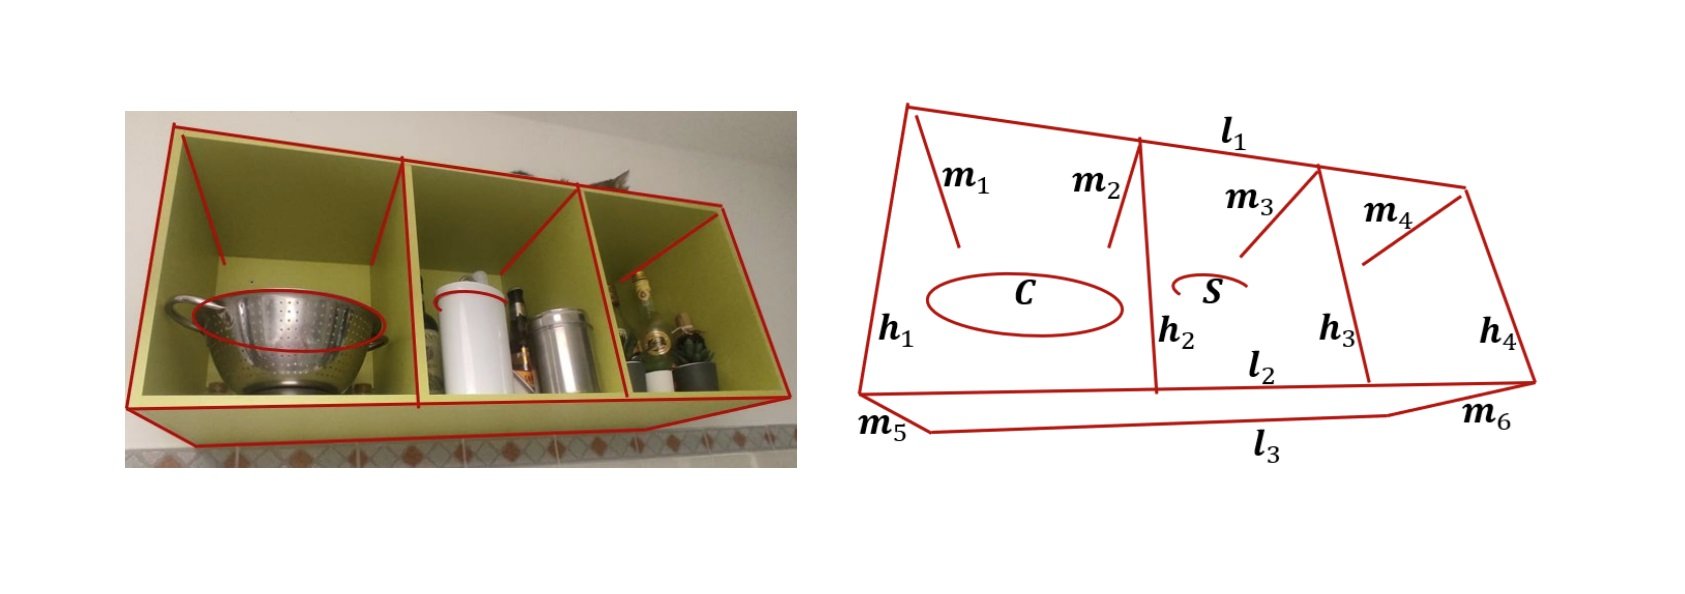
\includegraphics[width=1\linewidth]{scene.jpg}
\caption{\label{fig:scene}Presented scene.}
\end{figure}

The image visible in Figure \ref{fig:scene} displays a scene with a rectangular parallelepiped, taken by an uncalibrated, zero skew camera, whose calibration matrix depends on four unknown parameters.
Several sets of lines are visible and their images are extracted, among with images of a circumference and an unknown horizontal curve.\\
The report is split as such:
\begin{itemize}
    \item\textbf{Theory}: Theoretical solutions to the given problems, with assumptions and solutions based on the given setup.
    \item\textbf{Practice}: MATLAB implementation of the theoretical solutions, along with preprocessing, feature extraction techniques exploited and resuting plots.
\end{itemize} 
All solutions, plots and data computed in the following document can be directly checked and evaluated through MATLAB via the provided live script file "\textbf{homework.mlx}". All results and useful data is provided in \textit{".mat"} files along with the live script.


\chapter{Theory}

\section*{Theory Requests}

\begin{enumerate}
    \item From the \( l_i \) and \( m_j \) lines, find the vanishing line \( l'_{\infty} \) of the horizontal plane.
    \item Using the results of the previous point, find a (Euclidean) rectification mapping \( H_R \) for a horizontal plane (e.g., the lower horizontal face of the parallelepiped), and compute the depth \( m \) of the parallelepiped.
    \item From the results of the previous points, use the lines \( h_i \) to find the calibration matrix \( K \).
    \item Using the results of the previous points, determine the height \( h \) of the parallelepiped.
    \item Using \( S \) and the results of previous points, compute the X-Y coordinates of a dozen points (at your choice) of the unknown horizontal curve.
    \item Using \( K \), localize the camera with respect to the parallelepiped.
\end{enumerate}

\newpage
\section{Request 1: Vanishing Line \( l'_\infty \)}

\noindent
The vanishing line \( l'_\infty \) represents the image of the line at infinity \( l_\infty \). This line serves as the collection of all points at infinity.

\noindent
When two parallel lines intersect, their meeting point lies at infinity in the direction they share. The vanishing point is the projection of this point at infinity onto the image plane. Consequently, since parallelism isn't regularly preserved in a prospective image, to identify the vanishing line, we only need to compute two vanishing points from lines that would be parallel in a canonical 3D space.

\noindent
Since all \( l_i \) lines are parallel to one another, and the same holds for the \( m_j \) lines, we can select two lines from each set, choosing \( l_1 \) and \( l_2 \) from the \( l_i \) group, and \( m_1 \) and \( m_2 \) from the \( m_j \) group.

\noindent
To compute the vanishing points \( v_l \) and \( v_m \), we determine the intersections of \( l_1 \) with \( l_3 \), and \( m_1 \) with \( m_6 \) to then derive the vanishing line \( l'_\infty \) from the cross product of the two vanishing points in homogeneous coordinates:
\[
l_1^T \times v_l = 0;  
\]
\[
l_3^T \times v_l = 0;  
\]
\[
m_1^T \times v_m = 0;  
\]
\[
m_6^T \times v_m = 0;  
\]
\[
l'_\infty = v_l \times v_m;  
\]
Specifically, in this case, the vanishing line represents the locus of the vanishing points for the planar section of possible parallel lines formed by \( l_1 \) and \( l_3 \), and the planar section of possible parallel lines formed by \( m_1 \) and \( m_6 \) of the parallelepiped. These two sections define the perspective projections of the parallel lines in their respective groups, where each set of parallel lines shares a common vanishing point. The intersection of these vanishing points, as computed from the cross product of their homogeneous coordinates, defines the vanishing line \( l'_\infty \). This line acts as the boundary where the projection of all lines parallel to the two sets—\( l_i \) and \( m_j \)—converge, marking the transition to infinity in the image plane. 

\newpage
\section{Request 2: Rectification Mapping \( H_R \) and depth \(m\)}

\noindent
In order to compute the Euclidean Rectification Mapping $H_R$, we need to consider the vanishing line computed in point 2.1, along with the extracted matrix $C$ of the conic. To solve such problem, we need to determine the circular points \((I^{\prime}, J^{\prime})\). We know that the intersection of the image of the conic \(C^{\prime}\) and the vanishing line consists of two points, which are the images of the circular points \(I^{\prime}\) and \(J^{\prime}\).

\noindent
To find \(I^{\prime}\) and \(J^{\prime}\), we solve the following equation:

\[
l^{\prime}_{\infty} \cdot C^{\prime} = 0  
\]

\noindent
This yields two conjugate solutions, corresponding to the circular points. Using these, the image of the conic dual to the circular points is given by:

\[
C^{*}_{\infty}{}^{\prime} = I^{\prime}J^{\prime T} + J^{\prime}I^{\prime T}  
\]

\noindent
Next, we apply singular value decomposition (SVD) to the image of the conic dual to the circular points to obtain the matrix \(U\), and the rectifying transformation matrix \(H_{R}\) (named $T$ in the MATLAB section) can be obtained consequently:

\[
\text{svd}(C^{*}_{\infty}{}^{\prime}) = U \begin{bmatrix} a & 0 & 0 \\ 0 & b & 0 \\ 0 & 0 & 0 \end{bmatrix} U^{T}  
\]
\[
H_{R} = \begin{bmatrix} \frac{1}{\sqrt{a}} & 0 & 0 \\ 0 & \frac{1}{\sqrt{b}} & 0 \\ 0 & 0 & 1 \end{bmatrix} U^{T}  
\]

\noindent
Finally, to determine the depth \(m\) of the parallelepiped, we compute the proportion between Euclidean distance in pixels and real-model meters. This is possible because we know that any line \(1 = 1\) meter.

\noindent
To achieve this, we find the intersection points of a line \(l_{i}\) with two lines \(m_{j}\), obtaining the vertexes \(p1\), \(p2\), \(p3\), \(p4\) of the base of the parallelepiped (if not already available by data).

\noindent
The rectified points \(p1^{\prime}\), \(p2^{\prime}\), \(p3^{\prime}\), \(p4^{\prime}\) with respect to the horizontal plane are obtained by rectifying through \(H_{R}\) ($T$) by:

\[
p1^{\prime} = H_{R} \times p1^{T} 
\]
\[
p2^{\prime} = H_{R} \times p2^{T} 
\]
\[
p3^{\prime} = H_{R} \times p3^{T} 
\]
\[
p4^{\prime} = H_{R} \times p4^{T} 
\]

\noindent
Considering that \(p1^{\prime}\), \(p2^{\prime}\) are the points delimiting line \(l_{2}\) We can then compute the depth $m$ by proportion with respect to real life metrics and observed euclidean distances in the rectified space. The meters-to-pixels scaling can be computed as:
\[
\text{scaling}_{px/m} = \frac{\text{dist}(p1^{\prime}, p2^{\prime})}{1\,\text{m}}  
\]

We can then evaluate directly depth m from points \(p1^{\prime}\), \(p3^{\prime}\), delimiting line \(m_{5}\), as:

\[
m = \frac{\text{dist}(p1^{\prime}, p3^{\prime})}{\text{scaling}_{px/m}}  
\]

\newpage
\section{Request 3: Calibration matrix \(K\)}

\noindent
Since the camera is known to be zero skew, i.e. the axes of the camera sensor are perfectly orthogonal and the pixels on the image sensor are arranged in a perfect rectangular grid, there are only four unknowns in the calibration matrix \(K\):
\[
K = \begin{bmatrix} f_{x} & 0 & U_{0} \\ 0 & f_{y} & V_{0} \\ 0 & 0 & 1 \end{bmatrix}  
\]

\noindent
The image of the absolute conic \(\omega\) can be considered from the calibration matrix \(K\) by:
\[
\omega = (KK^{T})^{-1}  
\]

\noindent
Therefore, calibration matrix \(K\) can be found considering a rectified face and an orthogonal vanishing point to it. For this, we consider the rectifying homography \(T\) ($H_R$) from the previous point, its inverse \(T = T^{-1} = \left[ t_{1} ~~ t_{2} ~~ t_{3} \right]\), and the orthogonal vanishing point from lines \(h_{i}\), which can be evaluated as the cross product of two \(h_{i}\) as showed for lines \(l_{i}\) or \(m_{j}\) in section 2.1. We also consider the vanishing points \(v_{l}\), \(v_{m}\) from previous sections.

We can then find \(\omega\) solving the system of equations derived from vanishing point ortogonality and rectification conditions between \(\omega\) and \(T^{-1}\):
\[
v_{l}^{T} \omega v_{h} = 0
\]
\[
v_{m}^{T} \omega v_{h} = 0  
\]
\[
t_{1}^{T} \omega t_{2} = 0  
\]
\[
t_{1}^{T} \omega t_{1} - t_{2}^{T} \omega t_{2} = 0  
\]

\noindent
By solving this system numerically for the parameters \(f_{x}\) \(f_{y}\) \(u_{0}\) \(v_{0}\), we determine \(\omega\) and its parameters. The calibration matrix \(K\) is then derived by applying the Cholesky factorization of \(\omega^{-1} = KK^{T}\).



\newpage
\section{Request 4: Height \(h\)}

\noindent
Starting from the calibration matrix \(K\) obtained from section 2.3, and the image of the absolute conic \(\omega\) from the previous step, we can compute the circular points of the vertical plane considering the vanishing line of the vertical plane.
We already have the vanishing points required to compute it as \(v_{l}\), \(v_{h}\), so we can compute the vanishing line as:
\[
l^{\prime}_{1\infty} = V \times v_{1}  
\]

\noindent
We consider \(v_{l}\) and \(v_{h}\) to evaluate it used because the plane of interest contains the lines \(l_{i}\) and \(h_{j}\). Circular points \(I^{\prime}_{1}\) and \(J^{\prime}_{1}\) can be computed as the intersection between \(\omega\) and the vanishing line \(l^{\prime}_{1\infty}\). This corresponds to solve a system of equations.
The equations for the first circular point \(I^{\prime}_{1}\) are:
\[
I^{\prime}_{1} \times l^{\prime}_{1\infty} = 0  
\]
\[
I^{\prime T}_{1} \omega I^{\prime}_{1} = 0  
\]

\noindent
The same process is repeated for the second circular point \(J^{\prime}_{1}\).

\noindent
Once both circular points are determined, as for previous sections we compute the image of the conic dual to the circular points \(I^{\prime}_{1}\) and \(J^{\prime}_{1}\):
\[
C^{\star}_{1\infty} = I^{\prime}_{1} J^{\prime T}_{1} + J^{\prime}_{1} I^{\prime T}_{1}  
\]

\noindent
By applying singular value decomposition (SVD) to the image of the conic dual to the circular points, we then obtain the matrix \(U\) and a new rectification matrix $H_{Rvert}$ for the vertical plane, in the same way from section 2:
\[
\text{svd}(C^{\star}_{1\infty}) = U \begin{bmatrix} a & 0 & 0 \\ 0 & b & 0 \\ 0 & 0 & 0 \end{bmatrix} U^{T}  
\]
\[
H_{Rvert} = \begin{bmatrix} \frac{1}{\sqrt{a}} & 0 & 0 \\ 0 & \frac{1}{\sqrt{b}} & 0 \\ 0 & 0 & 1 \end{bmatrix} U^{T}  
\]

\noindent
Finally, to determine the height \(h\) of the parallelepiped, we compute the ratio between pixels and meters in the same way we computed it to find depth $m$.

\noindent
Since we already have two points for the line \(l_{2}\), namely \(p1\), \(p2\), we only need one additional point \((p5\) that forms a vertical line \(h_{i}\) with either of the two points, to define the height \(h\). We then compute the rectified points \((p1^{\prime}\), \((p2^{\prime}\) and \((p5^{\prime}\) with respect to the vertical plane:
\[
p1^{\prime} = H_{Rvert} \times p1^{T} 
\]
\[
p2^{\prime} = H_{Rvert} \times p2^{T} 
\]
\[
p5^{\prime} = H_{Rvert} \times p5^{T} 
\]

The scaling factor considering line \(l_{i}\), as before, is computed as:
\[
\text{scaling}_{px/m} = \frac{\text{dist}(p1^{\prime}, p2^{\prime})}{1\,\text{m}}  
\]

We can then evaluate directly height h from points \(p1^{\prime}\), \(p5^{\prime}\) as:

\[
h = \frac{\text{dist}(p1^{\prime}, p5^{\prime})}{\text{scaling}_{px/m}}  
\]

\newpage
\section{Request 5: Rectification of \(S\)}

\noindent
For each point \(s_{i}\), where \(i = 1, \dots, 12\), we need to satisfy the following equation:
\[
S \times s_{i} = 0  
\]

\noindent
This ensures that each point \(s_{i}\) lies on the curve \(S\). To find the corresponding X-Y coordinates of the horizontal curve with respect to the horizontal plane delimited by lines \(m_{5}\), \(m_{6}\), we apply the rectification matrix \(H_{R}\) (Matrix $T$):
\[
S_{i} = H_{R} \times s_{i}  
\]

\noindent
This way, we obtain the homogeneous X-Y coordinates for each selected point, after normalizing w.r.t. the third coordinate of each point \(S_{i}\).

\newpage
\section{Request 6: Camera Localization}

\noindent
From theory, homography \(H\) can be expressed as the product between the calibration matrix \(K\) and the matrix composed of the rotation vectors \(r_{1}\), \(r_{2}\) and the translation vector \(o_{\pi}\) with respect to the reference plane \(\pi\) of the subject:
\[
H = K \left[ r_{1} \quad r_{2} \quad o_{\pi} \right];
\]

\noindent
The vectors \(r_{1}\) and \(r_{2}\) are expected to be orthogonal by definition.
As a result, the camera's pose can be evaluated from \(H\) and \(K\) given by:
\[
\left[ r_{1} \quad r_{2} \quad o_{\pi} \right] = K^{-1} H.
\]

\noindent
Since the reference plane \(\pi\) is the parallelepiped, and the homography \(H\) between the plane \(\pi\) and its image is the inverse of the rectification matrix \(H_{R}\) computed earlier (since \(H_{R}\) maps from the image to the plane), we can compute the camera's pose as:
\[
\left[ r_{1} \quad r_{2} \quad o_{\pi} \right] = K^{-1} H_{R}^{-1}  
\]



\newpage
\chapter{MATLAB Implementation}

\section*{MATLAB Implementation Requests}
\begin{enumerate}
    \item Consider the image \texttt{Look-outCat.png}. Using feature extraction techniques (including those already implemented in Matlab) plus possible manual intervention, extract the images of useful lines and both the image \( C \), of the circumference and the image \( S \) of the other planar curve.
    \item Write a Matlab program that implements the solutions to problems 1–6 and show the obtained results.
    \item Plot the rectified curve \( S \) and show different views of the recovered 3D model of the rectangular parallelepiped.
\end{enumerate}

\newpage
\section{MATLAB Request 1: Data Extraction}

\noindent
We first need to extract all marked information from the image, i.e., lines \( l_1, l_2, l_3, m_1, m_2\),
\(m_3, m_4, m_5, m_6, h_1, h_2, h_3, h_4 \), along with conic \( C \) and curve \( S \).\\
This translates into obtaining the line vectors for each, along with conic \( C \) Matrix and curve \( S \) point displacement.

Manual techniques were implemented in order to extract these information as follows:
\begin{itemize}
    \item lines l, m, h: the cross product between two points was computed and normalized with respect to the third variable to obtain the line vector.
    \item Conic C: Conic $C$ was defined using six points by constructing matrix $A$ from their coordinates and solving for the null space via Singular Value Decomposition (SVD). The conic parameters $[a, b, c, d, e, f]$ were extracted from the last column of $V$ in the SVD, forming the symmetric $3 \times 3$ conic matrix $C$.
    \item Curve S: 12 points were selected and extracted from the scene, for computation in further points of the project.
\end{itemize}

The functions \textbf{getpts} and \textbf{ginput(n)} were exploited to extract points from the source image manually.

This resulted in the following extracted scene:
\begin{figure}[H]
    \centering
    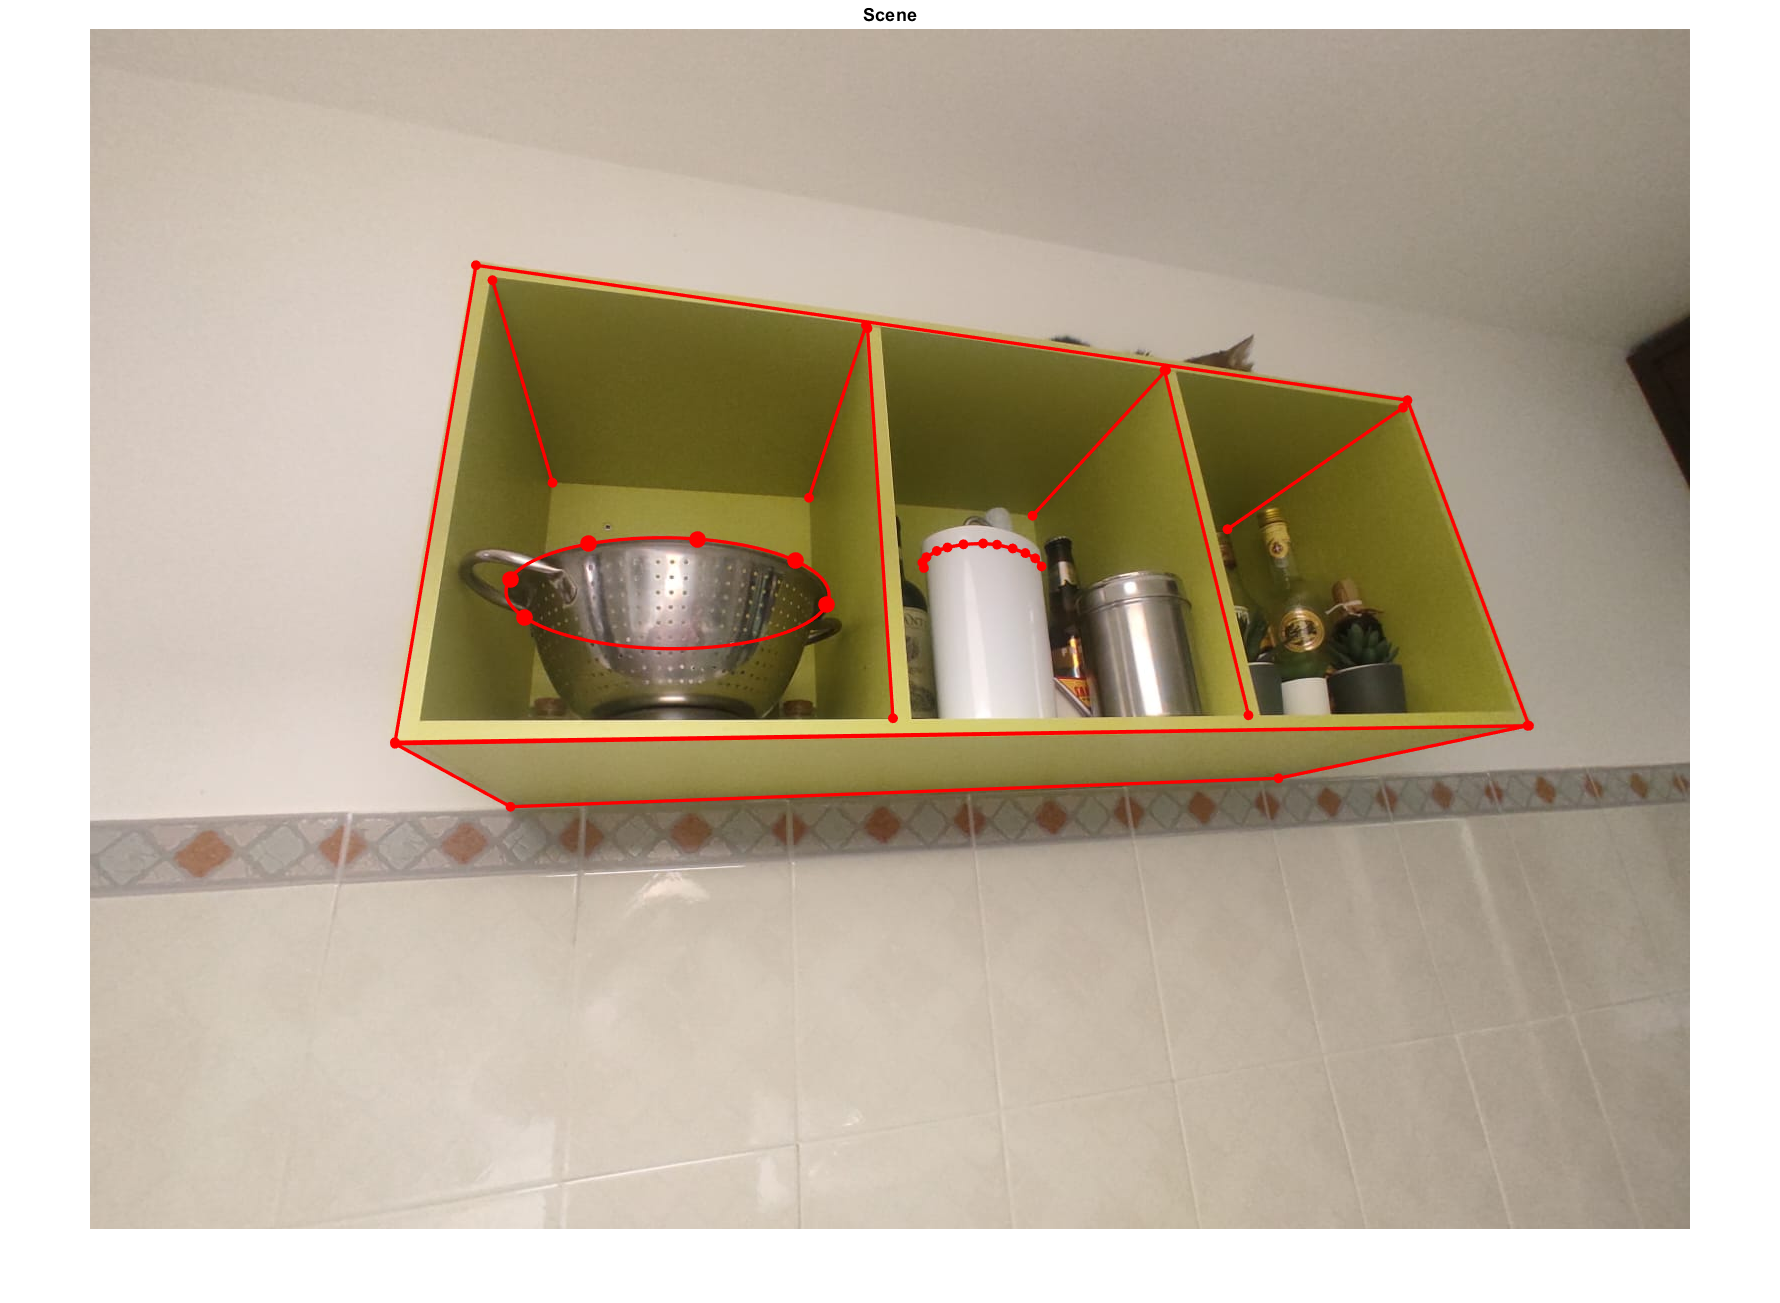
\includegraphics[width=0.75\linewidth]{Project Template/Images/extracted_scene.png}
    \caption{Extracted Scene}
    \label{fig:enter-label}
\end{figure}

Accordingly, some of the line equations were verified by intersecting them with the image borders, in order to ensure correctness of the computed vector:
\begin{figure}[H]
    \centering
    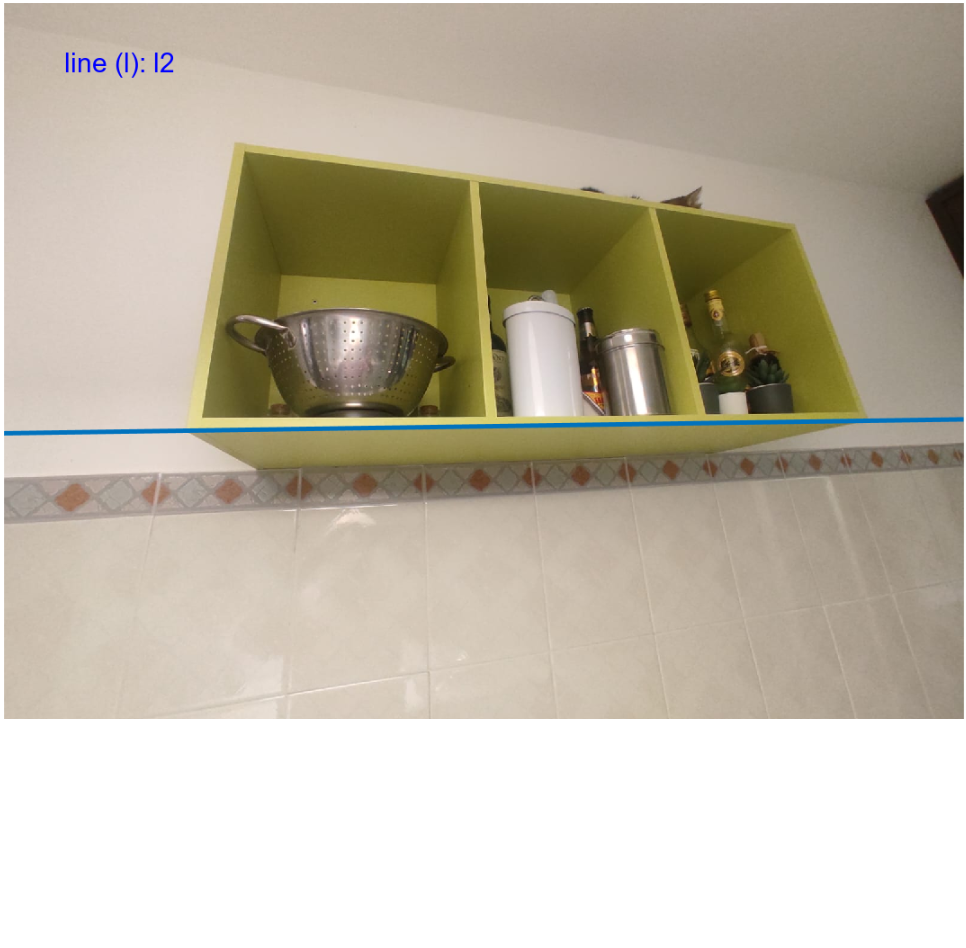
\includegraphics[width=0.5\linewidth]{Project Template/Images/l2.png}
    \caption{Line $l_2$}
    \label{fig:enter-label}
\end{figure}

\begin{figure}[H]
    \centering
    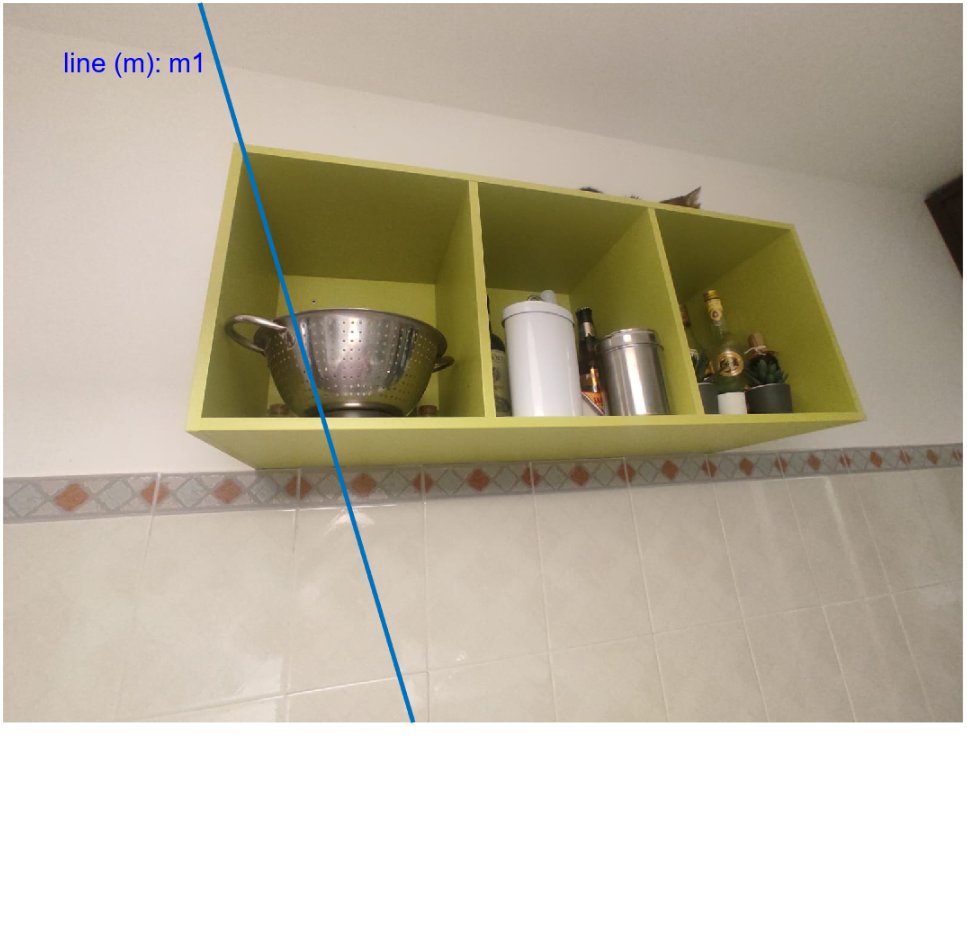
\includegraphics[width=0.5\linewidth]{Project Template/Images/m1.png}
    \caption{Line $m_1$}
    \label{fig:enter-label}
\end{figure}

\begin{figure}[H]
    \centering
    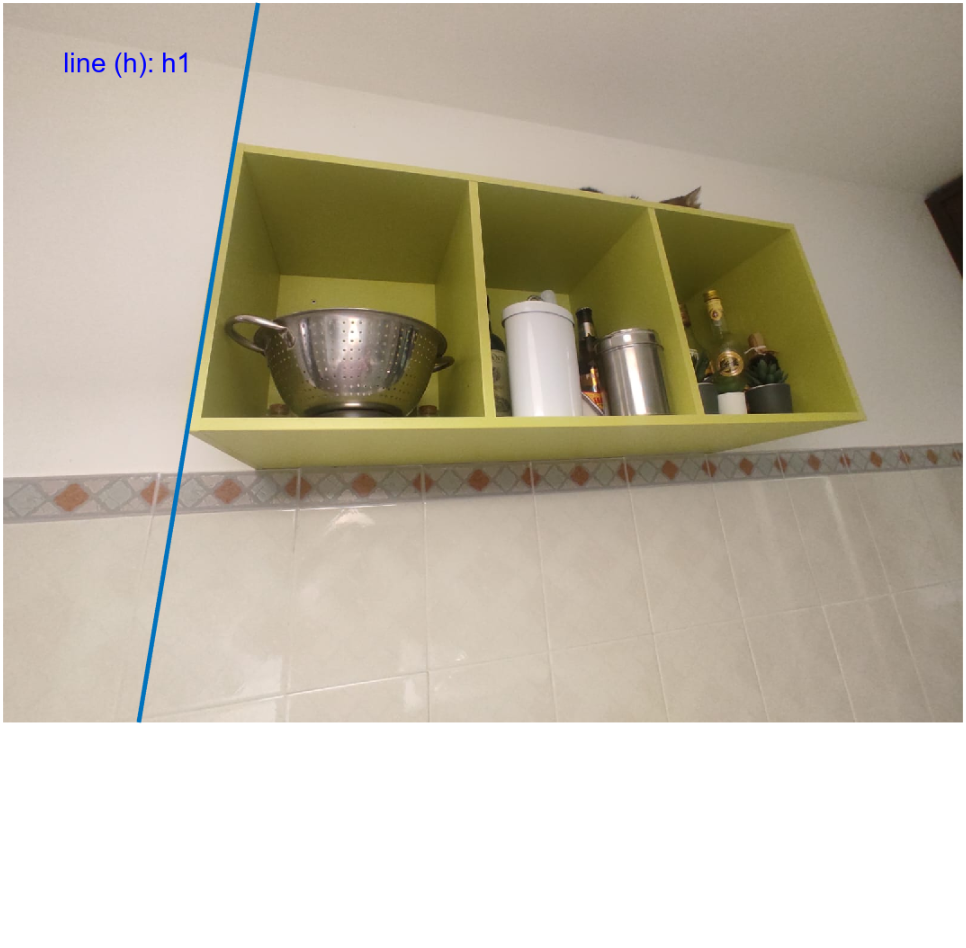
\includegraphics[width=0.5\linewidth]{Project Template/Images/h1.png}
    \caption{Line $h_1$}
    \label{fig:enter-label}
\end{figure}

\newpage
\section{MATLAB Request 2.1: }
Starting from the data extracted from the previous section, the vanishing points were computed as the intersection of pairs of parallel lines in the image. Specifically, the vanishing point $\mathbf{v}_{l_1l_3}$ was obtained by taking the cross product of the homogeneous coordinates of lines $\mathbf{l}_1$ and $\mathbf{l}_3$, while the vanishing point $\mathbf{v}_{m_1m_6}$ was computed as the cross product of lines $\mathbf{m}_1$ and $\mathbf{m}_6$. Both vanishing points were normalized to their homogeneous coordinates by dividing by their third component. 

The vanishing line $\mathbf{l}_{\infty}$ was then calculated as the cross product of the two vanishing points $\mathbf{v}_{l_1l_3}$ and $\mathbf{v}_{m_1m_6}$, and normalized to its homogeneous form. This line represents the horizon in the image plane, corresponding to the line at infinity in the projective space.

The computed vanishing points and the vanishing line were displayed for verification. The vanishing point from \( l_1 \) and \( l_3 \) was \( v_{l1\_l3} \), the vanishing point from \( m_1 \) and \( m_6 \) was \( v_{m1\_m6} \), and the vanishing line was \( l'_{\infty} \). 
This implementation successfully computed the vanishing line \( l'_{\infty} \) of the horizontal plane.
\begin{figure}[H]
    \centering
    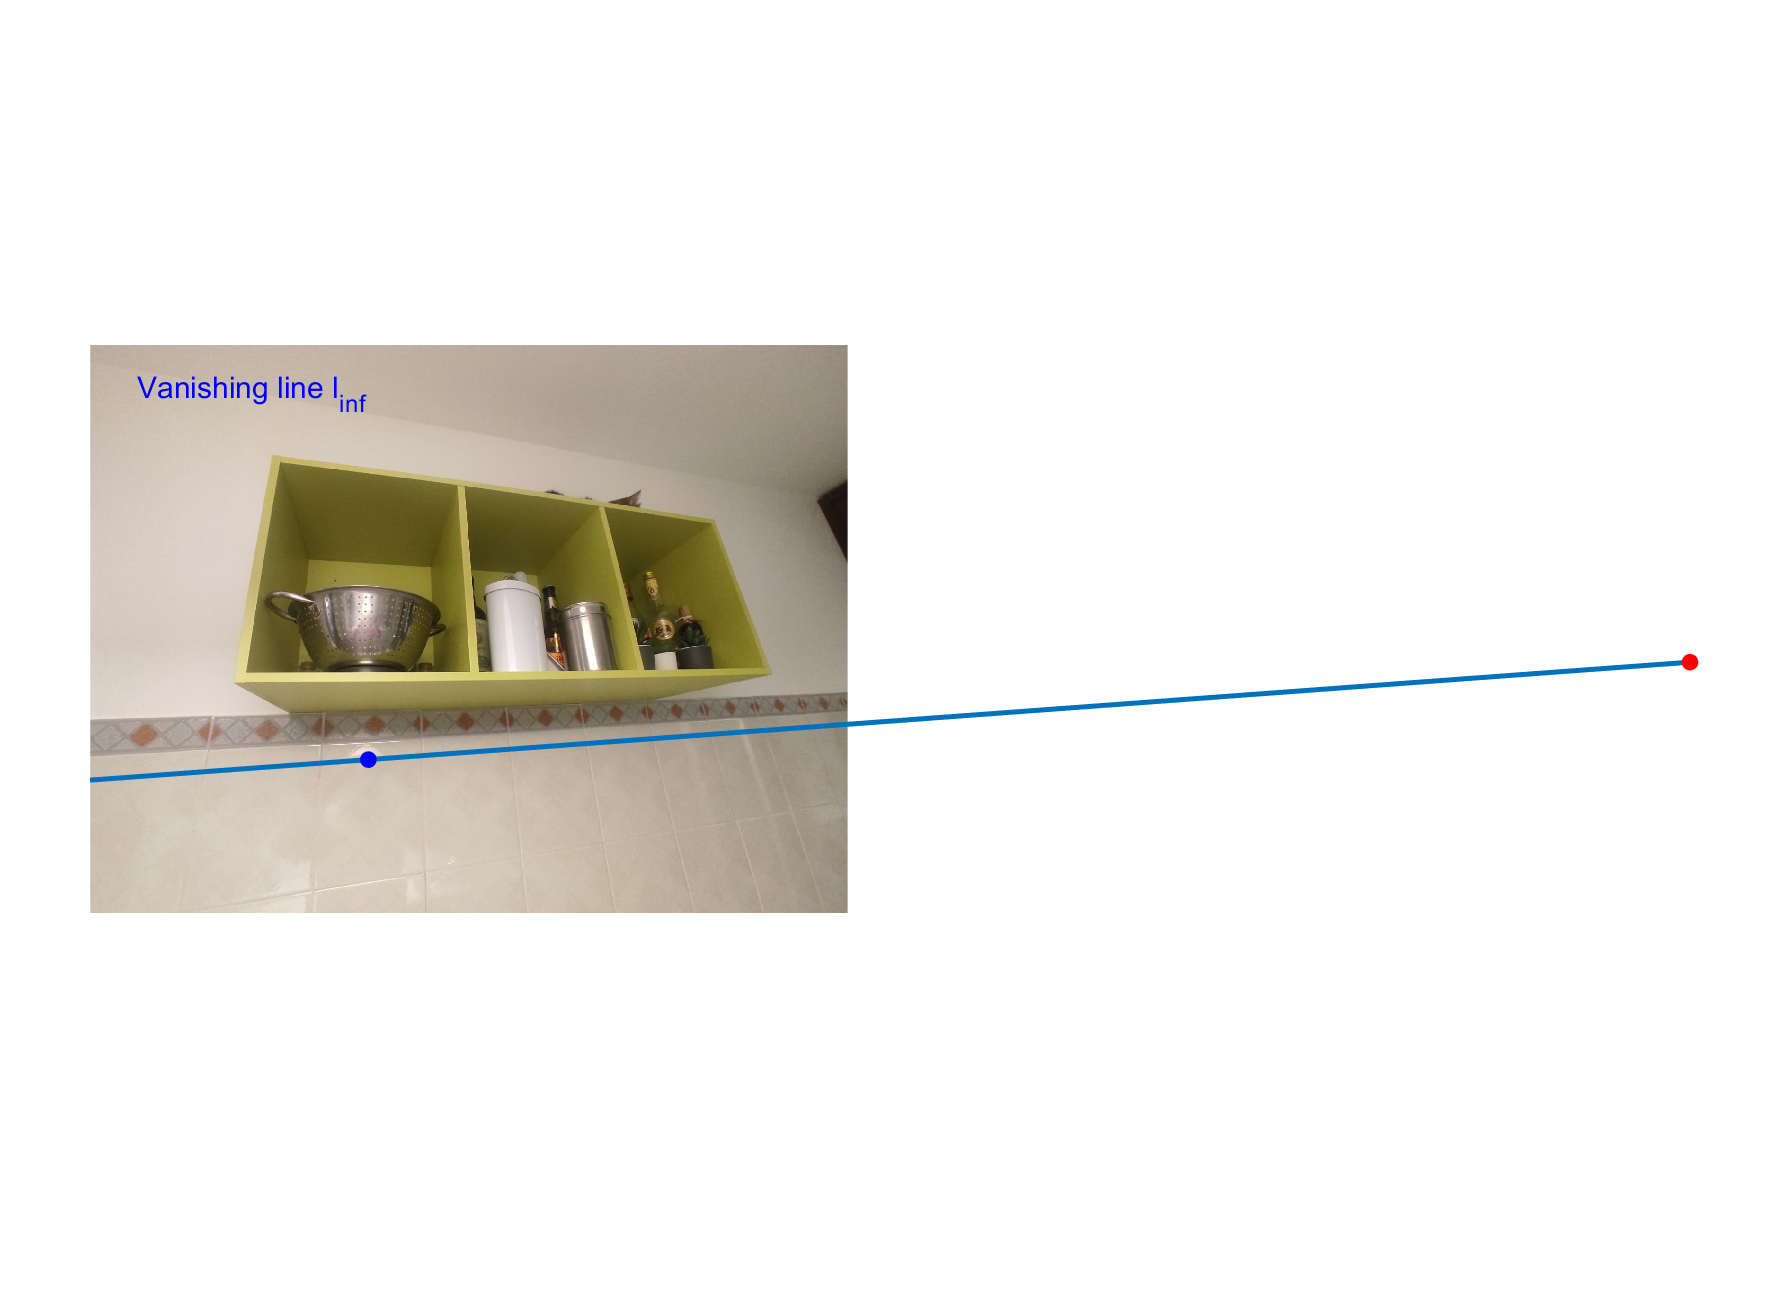
\includegraphics[width=0.78\linewidth]{Project Template/Images/vanishinglinepts.png}
    \caption{Vanishing line $l_{\infty}$}
    \label{fig:enter-label}
\end{figure}
The \textbf{blue} vanishing point was obtained from the intersection of lines \( m_1 \) and \( m_6 \), while the \textbf{red} vanishing point was obtained from the intersection of lines \( l_1 \) and \( l_3 \).\\

The following results were obtained:\\
Vanishing point from \( l_1 \) and \( l_3 \):
\[
\mathbf{v}_{l1\_l3} = \begin{bmatrix}
3380.0 \\
6706.0 \\
1
\end{bmatrix}
\]

Vanishing point from \( m_1 \) and \( m_6 \):
\[
\mathbf{v}_{m1\_m6} = \begin{bmatrix}
588.0953 \\
876.4468 \\
1
\end{bmatrix}
\]

Vanishing line (\( l_{\infty} \)):
\[
\mathbf{l}_{\infty} = \begin{bmatrix}
-0.0001 \\
-0.0011 \\
1
\end{bmatrix}
\]




\newpage
\section{MATLAB Request 2.2: }

The Euclidean rectification matrix \( T \) was computed by utilizing the vanishing line and a conic \( C \) extracted from the image. 

First, the extracted data was loaded, including vanishing lines, and vanishing points, from the previous sections of the code. 

Starting from matrix \( C \) of the conic, the Circular Points \( II \) and \( JJ \) were computed solving the system:
\[
a_{1} \cdot x^{2} + b_{1} \cdot x \cdot y + c_{1} \cdot y^{2} + d_{1} \cdot x + e_{1} \cdot y + f_{1} = 0 \quad 
\]
\[
l_{\infty,1} \cdot x + l_{\infty,2} \cdot y + l_{\infty,3} = 0 \quad 
\]

By solving for \textbf{x} and \textbf{y} through MATLAB's function \textbf{solve()}, since the image of the circular points are the intersection of the conic \( C \) with the vanishing line, I obtained the two complex Circular points.
For determining the image of the dual conic, matrix \(C^{*}_{\infty}{}^{\prime}\) was computed as:
\[
C^{*}_{\infty}{}^{\prime} = I^{\prime}J^{\prime T} + J^{\prime}I^{\prime T}
\]

From here, after computing a rectifying homography matrix \( H \) using the identity matrix and the vanishing line, following professor's Luca Magri method (from \textit{"Exercise Lecture E4D"}), a Rotation Matrix \textbf{U} was defined enforcing the ellipse \textit{C}'s axes equal. This exploited the \textbf{AtoG} function available as course material to convert the Conic's coefficient into geometrical parameters, in order to define matrix $U$'s angle constraints. Through a Scaling matrix \textbf{S} and a consequent affinity matrix \textbf{A} computed as \(K = U * S * U'\) the final transformation matrix \textbf{T} was obtained as composition of transformations as:
\[
T = A * H;
\]
The final values obtained are:
\[
\mathbf{T} = \begin{bmatrix}
1.3965 & -0.6187 & 0 \\
-0.6187 & 1.9656 & 0 \\
-8.0165\times10^{-5} & -0.0011 & 1
\end{bmatrix}
\]

The resulting Euclidean Rectification applied to the image yielded a scene (Figure \textbf{3.6}) giving a bottom view rectified perspective of the subject, preserving angles in order to compute the depth \textbf{m} requested. The ratio in pixel between the line \( m_5 \) and line \( l_1 \), known to be of length 1 meter, allowed to compute the depth, obtaining: 
\[
\mathbf{m} = 0.35458 m
\]

\begin{figure}[H]
    \centering
    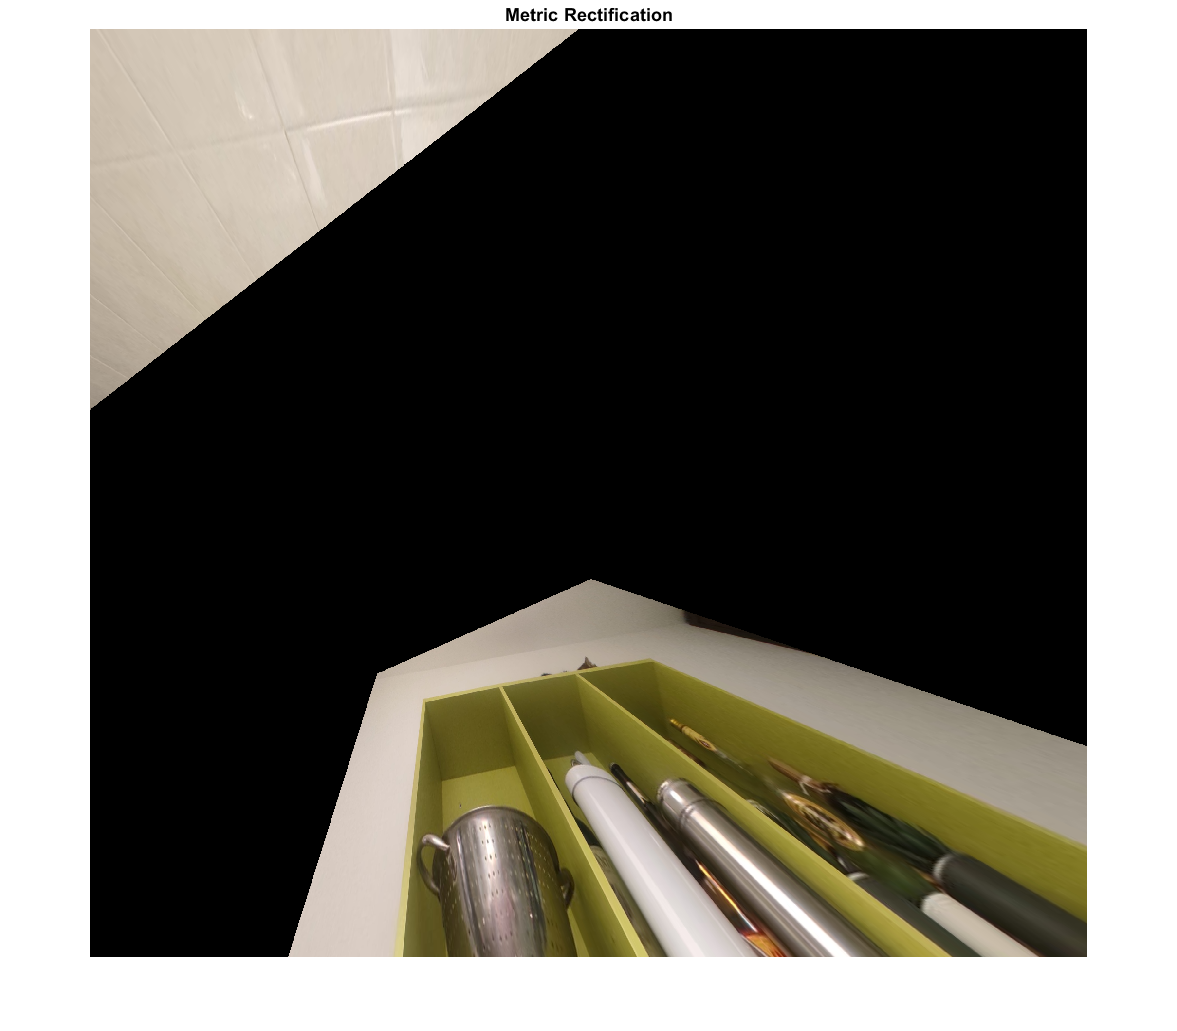
\includegraphics[width=0.8\linewidth]{Project Template/Images/metricrect.png}
    \caption{Euclidean Rectification from C}
    \label{fig:enter-label}
\end{figure}

\begin{figure}[H]
    \centering
    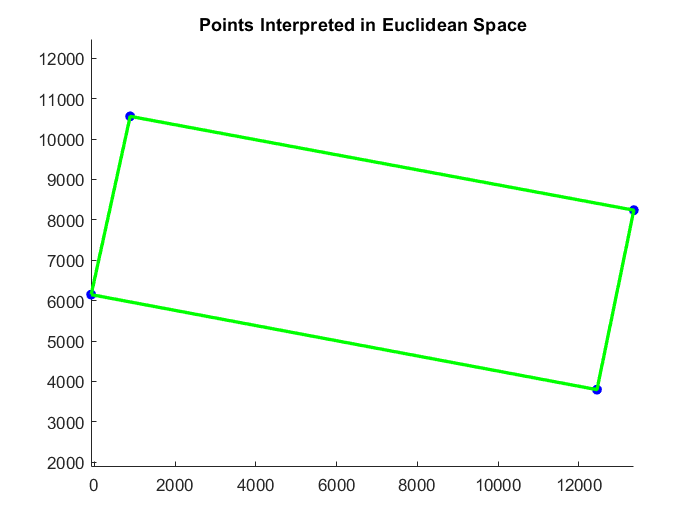
\includegraphics[width=0.5\linewidth]{Project Template/Images/basem.png}
    \caption{Base m of the subject}
    \label{fig:enter-label}
\end{figure}

We can verify how the metric transformation preserved the angles for the base composed of line \( m_5 \) and line \( m_6 \) from the plot in Figure 3.7, checking the reconstructed base of the parallelepiped.



\newpage
\section{MATLAB Request 2.3: }

In order to compute the calibration matrix \textbf{K} of the camera, we're required to compute the matrix from constraints on orthogonal vanishing points.
For determining the orthogonal vanishing point, lines $h_1$, $h_2$ were considered to obtain the vanishing point $v_{h1h2}$, the only one not computed in previous sections.
\\First, the columns of the inverse of matrix $T$ were considered as:
\[
\mathbf{T^{-1}} = [t_1, t_2, t_3]
\]

Using symbols $f_x$, $f_y$, $u_0$, $v_0$, matrices $\mathbf{K}$ and $\omega$ were defined symbolically. Following the theoretical solution, I employed four equations using previously calculated vanishing points and the rectification matrix's inverse from the prior problem. Indeed, through Zhang's Method for \textit{camera calibrations from known planar shapes}, we can define the following system of equations:
\[
\mathbf{v}_{l1l3}^\top \, \boldsymbol{\omega} \, \mathbf{v}_{h1h2} = 0
\]
\[
\mathbf{v}_{m1m6}^\top \, \boldsymbol{\omega} \, \mathbf{v}_{h1h2} = 0 
\]
\[
\mathbf{t}_1^\top \, \boldsymbol{\omega} \, \mathbf{t}_2 = 0
\]
\[
\mathbf{t}_1^\top \, \boldsymbol{\omega} \, \mathbf{t}_1 - \mathbf{t}_2^\top \, \boldsymbol{\omega} \, \mathbf{t}_2 = 0
\]


Through MATLAB's \texttt{vpasolve} function, in order to find a numerical solution to the four equations given the high number (4) of symbolic variables to solve, the calibration matrix \textbf{K} was evaluated resulting as:

\[
\mathbf{K} = \begin{bmatrix}
762.4680 & 0 & 805.3771 \\
0 & 778.8190 & 556.8548 \\
0 & 0 & 1
\end{bmatrix}
\]



\newpage
\section{MATLAB Request 2.4: }
To determine the vanishing line of the vertical plane as \( l1_{\inf_prime} \), the vanishing points \( v_{h1_h2} \) and \( v_{l1_l3} \) were crossed. 

To identify the circular points, as outlined in Problem 2.2, two equations were established using the symbolic variables \(x\) and \(y\):
\[
l1_{\inf_prime}^{T} \times I_{\text{prime}} = 0
\]
\[
I_{\text{prime}}^{T} \omega I_{\text{prime}} = 0
\]

These equations were solved through \textbf{solve()} for the symbolic variables \textbf{x, y}, in order to obtain once again the image of the circular points and the dual conic.
The rectifying transformation $\mathbf{H}_{Rvert}$ was then derived using Singular Value Decomposition of the conic dual to the circular points. After applying this transformation to rectify the image points at the vertexes of the considered vertical rectangle, this enabled to calculate the height in the same way depth was computed in the previous paragraph obtaining:
\[
\mathbf{h} = 0.38462 m
\]
\begin{figure}[H]
    \centering
    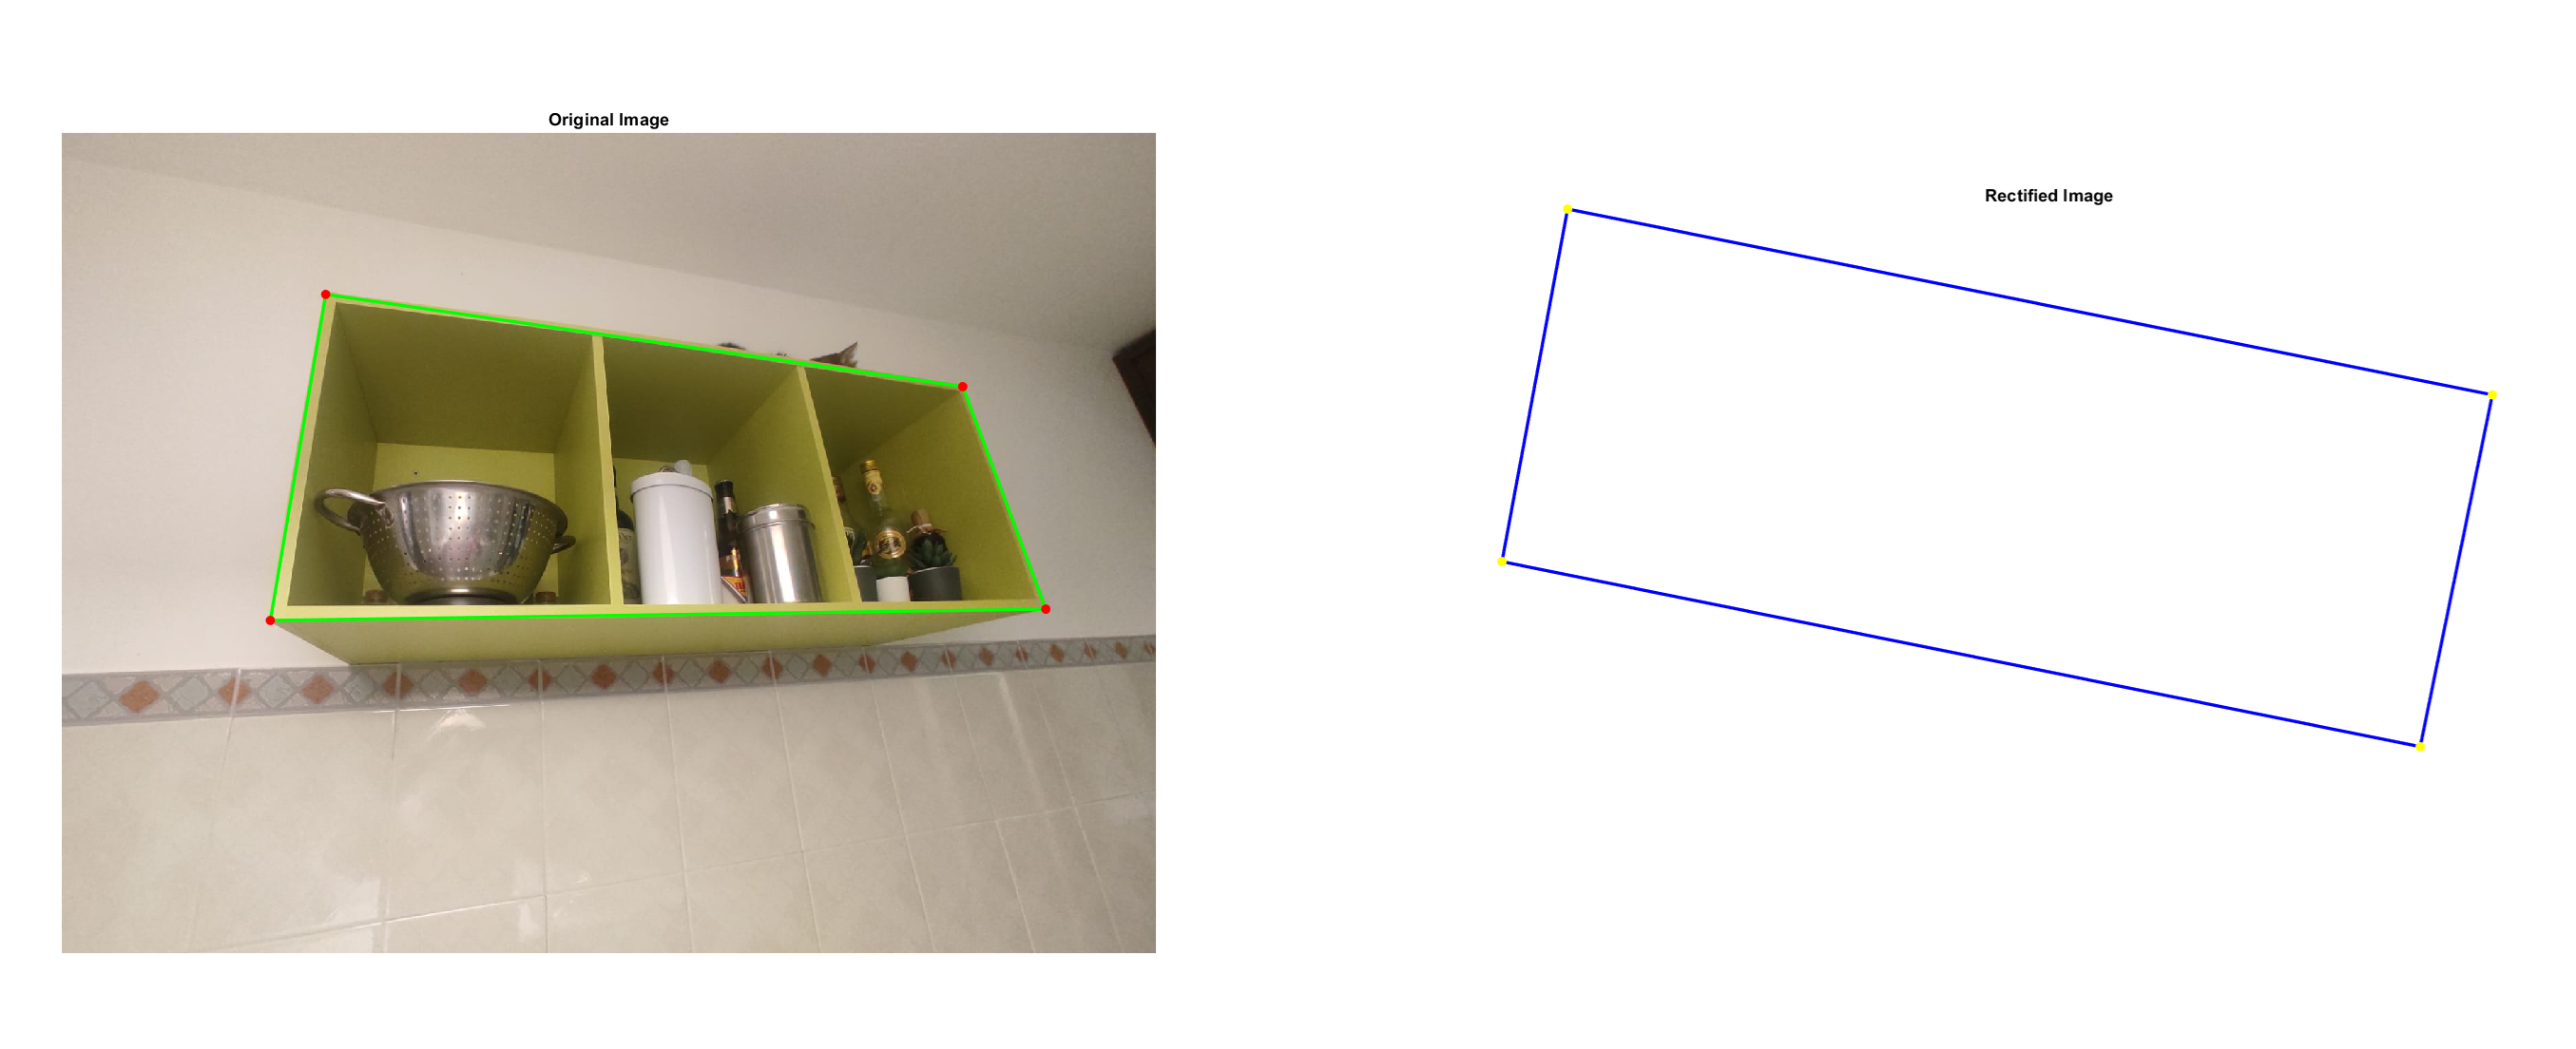
\includegraphics[width=0.9\linewidth]{Project Template/Images/point4.png}
    \caption{Rectified Vertical Plane}
    \label{fig:enter-label}
\end{figure}

From the second subplot, we can observe how the rectified vertical plane of the parallelepiped preserves the angles as expected with little to no noise, allowing to compute the height correctly.


\newpage
\section{MATLAB Request 2.5: }
The Rectification of the 12 points of \textbf{S} is computed directly from matrix \textbf{T} obtained in the previous sections.
Transformation T mapping the lower side of the parallelepiped is applied to the points of \textbf{S} as:
\[
S_{i} = T * s_{i}
\]
This yields the X-Y coordinates:
\[
\mathbf{S_{rect}} = \begin{bmatrix}
2941.3517 & 1381.8627 \\
2851.1471 & 1310.1073 \\
2769.5589 & 1274.9302 \\
2682.4338 & 1249.9673 \\
2589.8124 & 1237.6670 \\
2521.8416 & 1246.5530 \\
2441.3100 & 1281.7297 \\
2389.3326 & 1333.0092 \\
2362.0393 & 1380.9353 \\
2349.8979 & 1455.6222 \\
2361.9884 & 1516.2134 \\
2398.9329 & 1570.0334
\end{bmatrix}
\]

\section{MATLAB Request 2.6: }
To obtain both rotation vectors and translation vector with respect to $\pi$, we solve the pose matrix from theory with matrix \textbf{K} and \textbf{T}, yielding:
\[
R = \left[ r_1 \quad r_2 \quad \alpha_r \right] = 
\begin{bmatrix}
0.9326 & 0.0965 & -1.0562 \\
-0.3587 & 0.9453 & -0.7149 \\
-0.03901 & -0.3113 & 1
\end{bmatrix}
\]

The resulting camera placement can be seen by plotting according to rotation vectors \(r_{1}\), \(r_{2}\) and the translation vector \(o_{\pi}\) with respect to the reference plane \(\pi\) of the subject.
\begin{figure}[H]
    \centering
    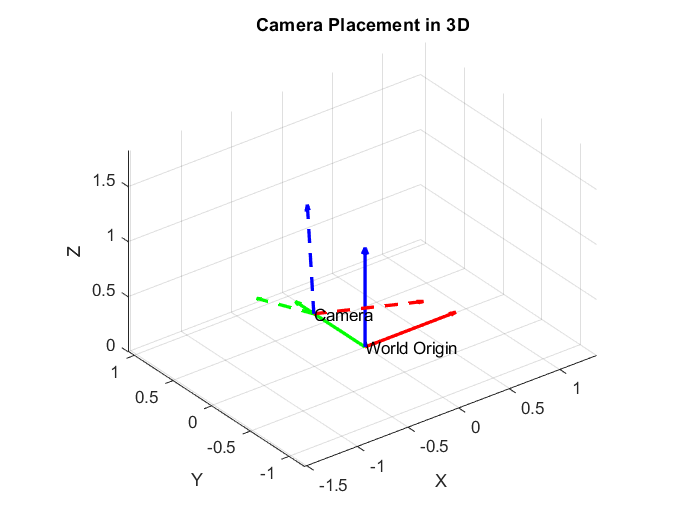
\includegraphics[width=0.5\linewidth]{Project Template/Images/cam.png}
    \caption{Camera Placement}
    \label{fig:enter-label}
\end{figure}
If we consider the plotted camera placement, we can spot how the X-axis of the camera (\textbf{red dotted line}) points right with respect to the X-axis of the world, while the Z-axis of the camera (\textbf{blue dotted line}) is slightly tilted. This suggest that the camera is being pointed tilted rightwards and slightly upwards, which is in accordance with the presented source view.

\newpage
\section{MATLAB Request 3: }
We can display curve \textbf{S} with the top-down view directly from the rectified points computed in MATLAB request 2.5:
\begin{figure}[H]
    \centering
    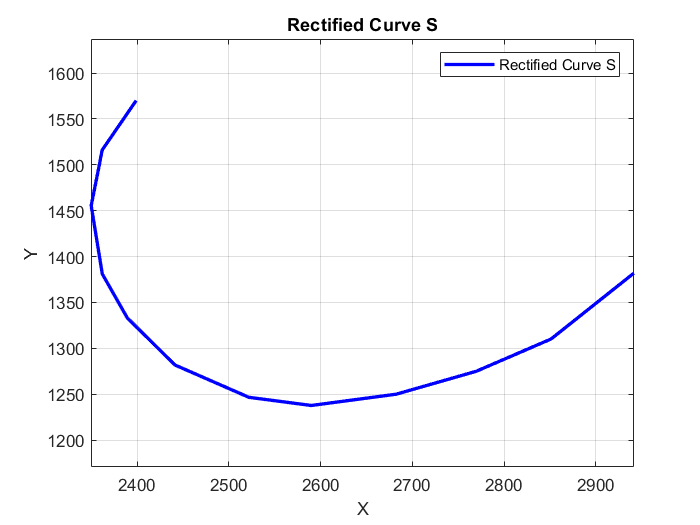
\includegraphics[width=0.5\linewidth]{Project Template/Images/s.png}
    \caption{Curve S}
    \label{fig:enter-label}
\end{figure}
As we can observe from the plot, the rectified image of the curve is compatible with the perspective we expect from the top down view of the considered object.

The 3D model of the parallelepiped can be built from the computed depths \textbf{m} and height \textbf{h} from the previous sections. Indeed, the 8 vertexes of the parallelepiped can be defined using $m$, $l$ and $h$ as variables, and the faces of the parallelepiped are consequently defined as sets of vertexes.
Three views are plotted respectively in order to show the 3D rendering of the model: \texttt{view(30, 30)}, \texttt{view(-30, 30)}, \texttt{view(60, 60)}.

\begin{figure}[H]
    \centering
    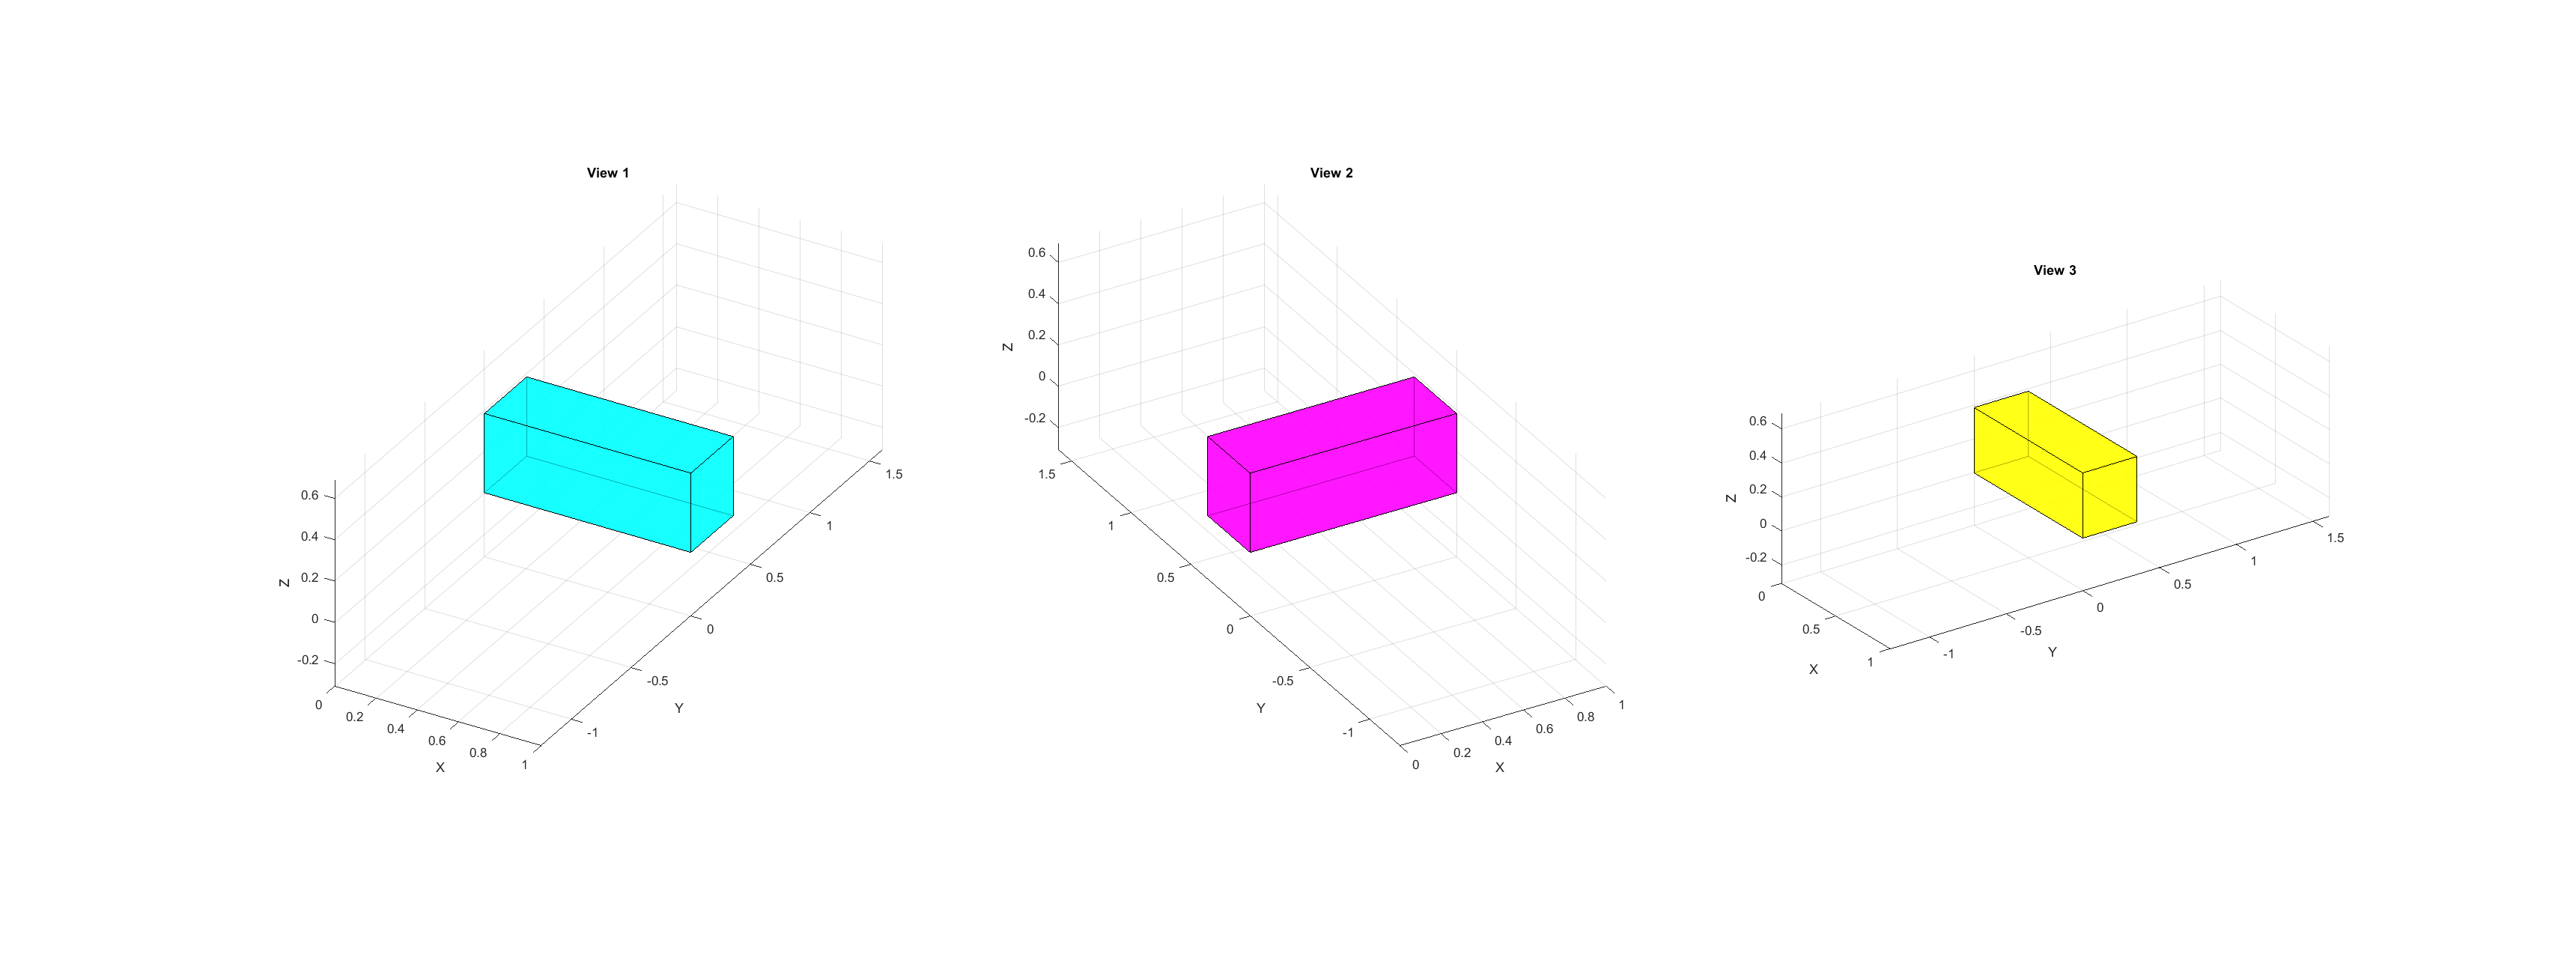
\includegraphics[width=1\linewidth]{Project Template/Images/3dview.png}
    \caption{3D View}
    \label{fig:enter-label}
\end{figure}

\chapter{Conclusions}
This Project allowed to apply Rectification and Reconstruction techniques to an existing, real scene of a parallelepiped object, in order to exploit Image Analysis methods to extract features, compute dimensions and transformation matrices, and perform the calibration of a zero-skew camera.\\
Both the original position of the camera with respect to the subject, and the 3D model of the parallelepiped itself, were reconstructed allowing to perceive the spacial disposition of the involved elements and their dimensions/orientations.
Further improvements could be implemented, for example considering Section 1 of the MATLAB section. Methods for automatic detection of lines were considered and tested, involving \textbf{houghpeaks()}, \textbf{houghlines()} and \textbf{Harris Detector Method}.\\
All solutions, plots and data computed in the following document can be directly checked and evaluated through MATLAB via the provided live script file "\textbf{homework.mlx}". All results and useful data is provided in \textit{".mat"} files along with the live script.

%-------------------------------------------------------------------------
%	APPENDICES
%-------------------------------------------------------------------------

\cleardoublepage
\addtocontents{toc}{\vspace{2em}} % Add a gap in the Contents, for aesthetics
\appendix
\chapter{References}
\begin{itemize}
    \item Theory Lectures from "IACV" Course - Politecnico di Milano
    \item Exercise Lectures from "IACV" Course - Politecnico di Milano
    \item MATLAB Documentation (upd. 2025, version M2023B)
\end{itemize}



\cleardoublepage

\end{document}
